% Options for packages loaded elsewhere
\PassOptionsToPackage{unicode}{hyperref}
\PassOptionsToPackage{hyphens}{url}
\documentclass[
]{article}
\usepackage{xcolor}
\usepackage[margin=1in]{geometry}
\usepackage{amsmath,amssymb}
\setcounter{secnumdepth}{-\maxdimen} % remove section numbering
\usepackage{iftex}
\ifPDFTeX
  \usepackage[T1]{fontenc}
  \usepackage[utf8]{inputenc}
  \usepackage{textcomp} % provide euro and other symbols
\else % if luatex or xetex
  \usepackage{unicode-math} % this also loads fontspec
  \defaultfontfeatures{Scale=MatchLowercase}
  \defaultfontfeatures[\rmfamily]{Ligatures=TeX,Scale=1}
\fi
\usepackage{lmodern}
\ifPDFTeX\else
  % xetex/luatex font selection
\fi
% Use upquote if available, for straight quotes in verbatim environments
\IfFileExists{upquote.sty}{\usepackage{upquote}}{}
\IfFileExists{microtype.sty}{% use microtype if available
  \usepackage[]{microtype}
  \UseMicrotypeSet[protrusion]{basicmath} % disable protrusion for tt fonts
}{}
\makeatletter
\@ifundefined{KOMAClassName}{% if non-KOMA class
  \IfFileExists{parskip.sty}{%
    \usepackage{parskip}
  }{% else
    \setlength{\parindent}{0pt}
    \setlength{\parskip}{6pt plus 2pt minus 1pt}}
}{% if KOMA class
  \KOMAoptions{parskip=half}}
\makeatother
\usepackage{color}
\usepackage{fancyvrb}
\newcommand{\VerbBar}{|}
\newcommand{\VERB}{\Verb[commandchars=\\\{\}]}
\DefineVerbatimEnvironment{Highlighting}{Verbatim}{commandchars=\\\{\}}
% Add ',fontsize=\small' for more characters per line
\usepackage{framed}
\definecolor{shadecolor}{RGB}{248,248,248}
\newenvironment{Shaded}{\begin{snugshade}}{\end{snugshade}}
\newcommand{\AlertTok}[1]{\textcolor[rgb]{0.94,0.16,0.16}{#1}}
\newcommand{\AnnotationTok}[1]{\textcolor[rgb]{0.56,0.35,0.01}{\textbf{\textit{#1}}}}
\newcommand{\AttributeTok}[1]{\textcolor[rgb]{0.13,0.29,0.53}{#1}}
\newcommand{\BaseNTok}[1]{\textcolor[rgb]{0.00,0.00,0.81}{#1}}
\newcommand{\BuiltInTok}[1]{#1}
\newcommand{\CharTok}[1]{\textcolor[rgb]{0.31,0.60,0.02}{#1}}
\newcommand{\CommentTok}[1]{\textcolor[rgb]{0.56,0.35,0.01}{\textit{#1}}}
\newcommand{\CommentVarTok}[1]{\textcolor[rgb]{0.56,0.35,0.01}{\textbf{\textit{#1}}}}
\newcommand{\ConstantTok}[1]{\textcolor[rgb]{0.56,0.35,0.01}{#1}}
\newcommand{\ControlFlowTok}[1]{\textcolor[rgb]{0.13,0.29,0.53}{\textbf{#1}}}
\newcommand{\DataTypeTok}[1]{\textcolor[rgb]{0.13,0.29,0.53}{#1}}
\newcommand{\DecValTok}[1]{\textcolor[rgb]{0.00,0.00,0.81}{#1}}
\newcommand{\DocumentationTok}[1]{\textcolor[rgb]{0.56,0.35,0.01}{\textbf{\textit{#1}}}}
\newcommand{\ErrorTok}[1]{\textcolor[rgb]{0.64,0.00,0.00}{\textbf{#1}}}
\newcommand{\ExtensionTok}[1]{#1}
\newcommand{\FloatTok}[1]{\textcolor[rgb]{0.00,0.00,0.81}{#1}}
\newcommand{\FunctionTok}[1]{\textcolor[rgb]{0.13,0.29,0.53}{\textbf{#1}}}
\newcommand{\ImportTok}[1]{#1}
\newcommand{\InformationTok}[1]{\textcolor[rgb]{0.56,0.35,0.01}{\textbf{\textit{#1}}}}
\newcommand{\KeywordTok}[1]{\textcolor[rgb]{0.13,0.29,0.53}{\textbf{#1}}}
\newcommand{\NormalTok}[1]{#1}
\newcommand{\OperatorTok}[1]{\textcolor[rgb]{0.81,0.36,0.00}{\textbf{#1}}}
\newcommand{\OtherTok}[1]{\textcolor[rgb]{0.56,0.35,0.01}{#1}}
\newcommand{\PreprocessorTok}[1]{\textcolor[rgb]{0.56,0.35,0.01}{\textit{#1}}}
\newcommand{\RegionMarkerTok}[1]{#1}
\newcommand{\SpecialCharTok}[1]{\textcolor[rgb]{0.81,0.36,0.00}{\textbf{#1}}}
\newcommand{\SpecialStringTok}[1]{\textcolor[rgb]{0.31,0.60,0.02}{#1}}
\newcommand{\StringTok}[1]{\textcolor[rgb]{0.31,0.60,0.02}{#1}}
\newcommand{\VariableTok}[1]{\textcolor[rgb]{0.00,0.00,0.00}{#1}}
\newcommand{\VerbatimStringTok}[1]{\textcolor[rgb]{0.31,0.60,0.02}{#1}}
\newcommand{\WarningTok}[1]{\textcolor[rgb]{0.56,0.35,0.01}{\textbf{\textit{#1}}}}
\usepackage{longtable,booktabs,array}
\usepackage{calc} % for calculating minipage widths
% Correct order of tables after \paragraph or \subparagraph
\usepackage{etoolbox}
\makeatletter
\patchcmd\longtable{\par}{\if@noskipsec\mbox{}\fi\par}{}{}
\makeatother
% Allow footnotes in longtable head/foot
\IfFileExists{footnotehyper.sty}{\usepackage{footnotehyper}}{\usepackage{footnote}}
\makesavenoteenv{longtable}
\usepackage{graphicx}
\makeatletter
\newsavebox\pandoc@box
\newcommand*\pandocbounded[1]{% scales image to fit in text height/width
  \sbox\pandoc@box{#1}%
  \Gscale@div\@tempa{\textheight}{\dimexpr\ht\pandoc@box+\dp\pandoc@box\relax}%
  \Gscale@div\@tempb{\linewidth}{\wd\pandoc@box}%
  \ifdim\@tempb\p@<\@tempa\p@\let\@tempa\@tempb\fi% select the smaller of both
  \ifdim\@tempa\p@<\p@\scalebox{\@tempa}{\usebox\pandoc@box}%
  \else\usebox{\pandoc@box}%
  \fi%
}
% Set default figure placement to htbp
\def\fps@figure{htbp}
\makeatother
% definitions for citeproc citations
\NewDocumentCommand\citeproctext{}{}
\NewDocumentCommand\citeproc{mm}{%
  \begingroup\def\citeproctext{#2}\cite{#1}\endgroup}
\makeatletter
 % allow citations to break across lines
 \let\@cite@ofmt\@firstofone
 % avoid brackets around text for \cite:
 \def\@biblabel#1{}
 \def\@cite#1#2{{#1\if@tempswa , #2\fi}}
\makeatother
\newlength{\cslhangindent}
\setlength{\cslhangindent}{1.5em}
\newlength{\csllabelwidth}
\setlength{\csllabelwidth}{3em}
\newenvironment{CSLReferences}[2] % #1 hanging-indent, #2 entry-spacing
 {\begin{list}{}{%
  \setlength{\itemindent}{0pt}
  \setlength{\leftmargin}{0pt}
  \setlength{\parsep}{0pt}
  % turn on hanging indent if param 1 is 1
  \ifodd #1
   \setlength{\leftmargin}{\cslhangindent}
   \setlength{\itemindent}{-1\cslhangindent}
  \fi
  % set entry spacing
  \setlength{\itemsep}{#2\baselineskip}}}
 {\end{list}}
\usepackage{calc}
\newcommand{\CSLBlock}[1]{\hfill\break\parbox[t]{\linewidth}{\strut\ignorespaces#1\strut}}
\newcommand{\CSLLeftMargin}[1]{\parbox[t]{\csllabelwidth}{\strut#1\strut}}
\newcommand{\CSLRightInline}[1]{\parbox[t]{\linewidth - \csllabelwidth}{\strut#1\strut}}
\newcommand{\CSLIndent}[1]{\hspace{\cslhangindent}#1}
\setlength{\emergencystretch}{3em} % prevent overfull lines
\providecommand{\tightlist}{%
  \setlength{\itemsep}{0pt}\setlength{\parskip}{0pt}}
\usepackage{float}
\floatplacement{figure}{H}
\usepackage[numbers]{natbib}
\setlength{\bibsep}{1em}
\usepackage{booktabs}
\usepackage{longtable}
\usepackage{array}
\usepackage{multirow}
\usepackage{wrapfig}
\usepackage{float}
\usepackage{colortbl}
\usepackage{pdflscape}
\usepackage{tabu}
\usepackage{threeparttable}
\usepackage{threeparttablex}
\usepackage[normalem]{ulem}
\usepackage{makecell}
\usepackage{xcolor}
\usepackage{bookmark}
\IfFileExists{xurl.sty}{\usepackage{xurl}}{} % add URL line breaks if available
\urlstyle{same}
\hypersetup{
  pdftitle={Application to air pollution forecasting},
  pdfauthor={Raphaela Azar; Sbonelo Gumede},
  hidelinks,
  pdfcreator={LaTeX via pandoc}}

\title{Application to air pollution forecasting}
\author{Raphaela Azar \and Sbonelo Gumede}
\date{2025-09-30}

\begin{document}
\maketitle

\section{Introduction}\label{introduction}

The World Health Organization estimated that approximately seven million
people die every year due to air pollution (Cape Town 2024). To manage
levels of air pollution, the City of Cape Town has built eleven air
quality monitoring (AQM) stations in Cape Town. These stations collect
data on particulate matter 10 \((\text{PM}_{10})\), particulate matter
2.5 \((\text{PM}_{2.5})\), sulphur dioxide \((\text{SO}_{2})\), nitrogen
dioxide \((\text{NO}_{2})\), ozone \((\text{O}_{3})\), hydrogen sulphide
\((\text{H}_{2}\text{S})\), carbon monoxide \((\text{CO})\), benzene
\((\text{C}_{6}\text{H}_{6})\), and lead \((\text{Pb})\) (Cape Town
2024). Air pollution data for Cape Town can be found on the City of Cape
Town open data portal (Cape Town 2015).

The Table View station was chosen for this project. This is because it
had the fewest missing observations. The data consist of our response
variable, nitrogen dioxide \((\mu g / m^3)\), and explanatory variables,
sulphur dioxide \((\mu g / m^3)\), particulate matter 10
\((\mu g / m^3)\), and wind speed \((m/s)\) from 01/01/2019 to
31/12/2019, measured hourly at the Table View station.

\section{Exploratory data analysis}\label{exploratory-data-analysis}

\begin{longtable}[]{@{}lrrrrrrrr@{}}
\caption{Summary statistics of the air quality dataset from 01/01/2019
to 31/12/2019 measured hourly.}\tabularnewline
\toprule\noalign{}
& Min. & 1st Qu. & Median & Mean & SD & 3rd Qu. & Max. & NA \\
\midrule\noalign{}
\endfirsthead
\toprule\noalign{}
& Min. & 1st Qu. & Median & Mean & SD & 3rd Qu. & Max. & NA \\
\midrule\noalign{}
\endhead
\bottomrule\noalign{}
\endlastfoot
NO2 & 0.0 & 5.0 & 9.0 & 12.729 & 10.724 & 17.0 & 113.0 & 734 \\
PM10 & 0.0 & 12.0 & 17.0 & 19.824 & 12.302 & 24.0 & 158.0 & 298 \\
SO2 & 0.0 & 2.0 & 3.0 & 6.202 & 11.299 & 5.0 & 142.0 & 638 \\
Speed & 0.5 & 2.3 & 3.6 & 3.735 & 1.710 & 4.9 & 11.2 & 918 \\
\end{longtable}

All variables in this dataset are non-negative, and many observations
are missing. Some of the time series models we work with cannot handle
missing data directly, so we perform imputation. Initially, we tried
natural cubic splines, but some imputed values were negative because
splines are unconstrained, which is problematic for non-negative
variables. We then applied linear interpolation, which preserved the
statistical properties of the data reasonably well. However, linear
interpolation does not enforce smoothness across the time series. To
address this, we used Kalman filter-based interpolation via the
\texttt{na\_kalman()} function in the \texttt{imputeTS} package in
\texttt{R}. This method produces smooth, non-negative estimates and is
statistically optimal for estimating missing values in time series
(Corey Montella). It effectively leverages the temporal structure of the
data, resulting in imputed values that respect both the data's
continuity and its statistical properties. This uses a local level
model, which is the simplest structural time series (state space) model.

\begin{longtable}[]{@{}lrrrrrrrr@{}}
\caption{Summary statistics of the imputed air quality dataset from
01/01/2019 to 31/12/2019.}\tabularnewline
\toprule\noalign{}
& Min. & 1st Qu. & Median & Mean & SD & 3rd Qu. & Max. & NA \\
\midrule\noalign{}
\endfirsthead
\toprule\noalign{}
& Min. & 1st Qu. & Median & Mean & SD & 3rd Qu. & Max. & NA \\
\midrule\noalign{}
\endhead
\bottomrule\noalign{}
\endlastfoot
NO2 & 0.0 & 5.0 & 9.0 & 12.806 & 10.773 & 17.0 & 113.0 & 0 \\
PM10 & 0.0 & 12.0 & 17.0 & 19.679 & 12.200 & 24.0 & 158.0 & 0 \\
SO2 & 0.0 & 2.0 & 3.0 & 6.331 & 11.097 & 5.0 & 142.0 & 0 \\
Speed & 0.5 & 2.4 & 3.4 & 3.703 & 1.664 & 4.8 & 11.2 & 0 \\
\end{longtable}

Notice that the summary statistics did not change much after applying
the Kalman filter interpolation.

\begin{figure}
\centering
\pandocbounded{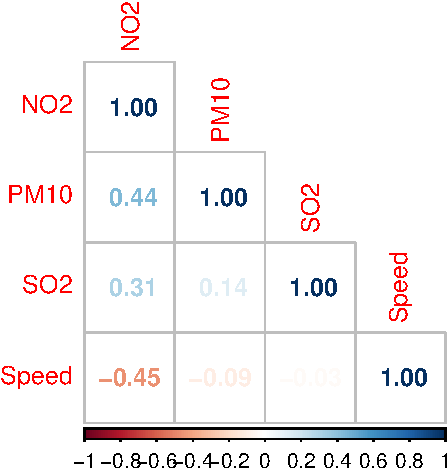
\includegraphics[keepaspectratio]{report_files/figure-latex/Correlation plot of the original data-1.pdf}}
\caption{Correlation plot of the air quality dataset from 01/01/2019 to
31/12/2019 measured hourly.}
\end{figure}

Our response variable \(\text{NO}_{2}\) appears to be moderately
positively correlated with \(\text{PM}_{10}\) and \(\text{SO}_{2}\), and
moderately negatively correlated with Speed. These are not ideal
explanatory variables since we typically would like them to be strongly
correlated with the response variable. The explanatory variables are
weakly correlated with one another, whether it be a positive or a
negative correlation. This is ideal since some models do not work well
with correlated explanatory variables, often leading to unstable point
estimates and inflated standard errors.

\begin{figure}
\centering
\pandocbounded{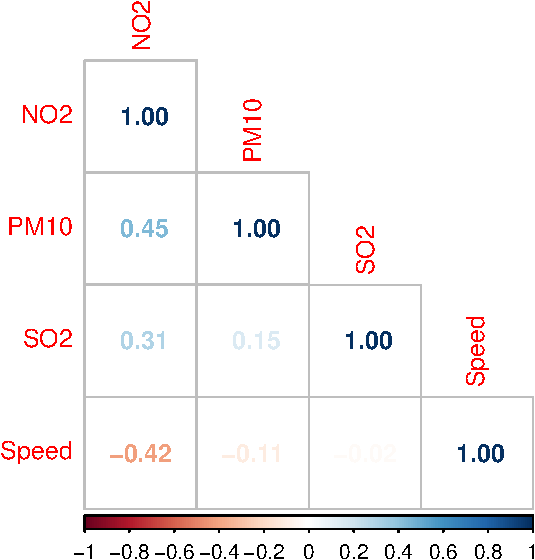
\includegraphics[keepaspectratio]{report_files/figure-latex/Correlation plot of the imputed data-1.pdf}}
\caption{Correlation plot of the imputed air quality dataset from
01/01/2019 to 31/12/2019 measured hourly.}
\end{figure}

Notice that the correlations between variables did not change much after
applying the Kalman filter interpolation.

\begin{figure}
\centering
\pandocbounded{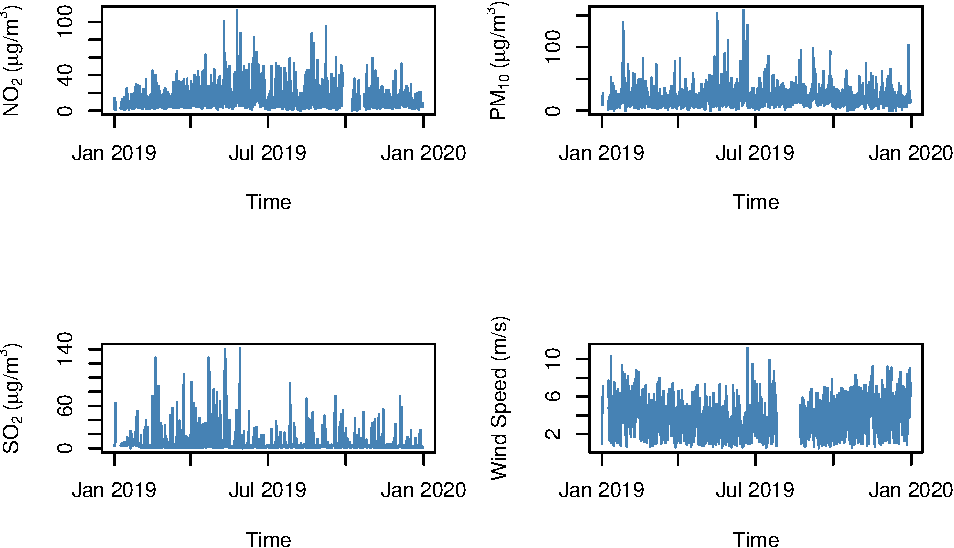
\includegraphics[keepaspectratio]{report_files/figure-latex/Scatter plots of the original data-1.pdf}}
\caption{Scatter plots of the air quality dataset from 01/01/2019 to
31/12/2019 measured hourly.}
\end{figure}

There seems to be a weak seasonal and trend component based on the time
series plots. There is no clear indication of a cyclical component.
There is random variation as usual. It is challenging to visually
identify the time series components since this is a noisy dataset.

\begin{figure}
\centering
\pandocbounded{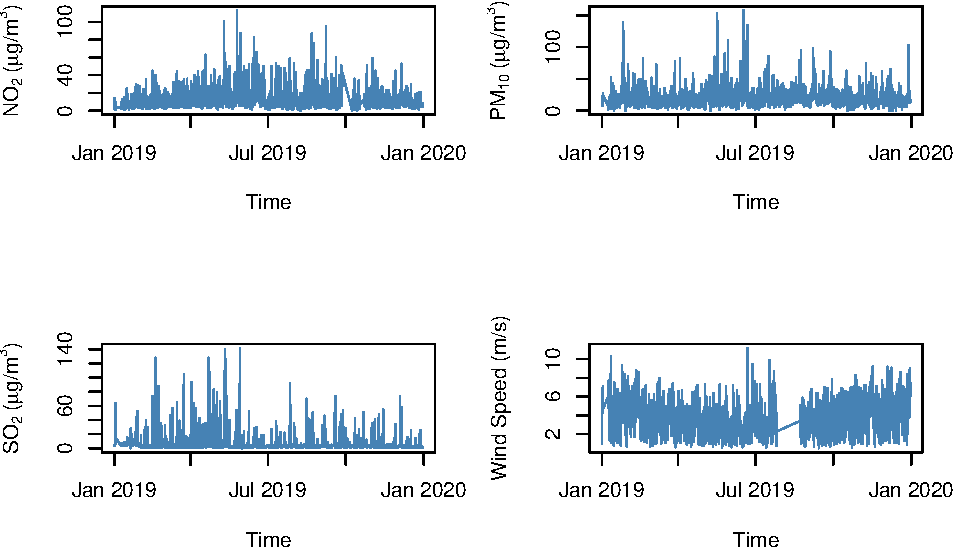
\includegraphics[keepaspectratio]{report_files/figure-latex/Scatter plots of the imputed data-1.pdf}}
\caption{Scatter plots of the imputed air quality dataset from
01/01/2019 to 31/12/2019 measured hourly.}
\end{figure}

Notice that the time series plots did not change much after applying the
Kalman filter interpolation.

\section{Model formulation}\label{model-formulation}

Let the window from 08/02/2019 at 00:00 to 15/02/2019 at 23:00 denote
our training set (response variable \(\mathbf{y}_{1}\) and design matrix
\(\mathbf{X}_{1}\)). And let the window from 16/02/2019 at 00:00 to
16/02/2019 at 23:00 denote our test set (response variable
\(\mathbf{y}_{2}\) and design matrix \(\mathbf{X}_{2}\)).

\subsection{Simple forecasting models}\label{simple-forecasting-models}

\texttt{Mean}: The prediction is the average value. The Mean method
\[\hat{y}_{2_{n_{1} + h}} = \sum_{i=1}^{n_{1}} \frac{y_{1_{i}}} {n_{1}}.\]

\texttt{Naive}: The prediction is the last observed value. The Naive
method \[\hat{y}_{2_{n_{1} + h}} = y_{1_{n_{1}}}.\]

\texttt{Seasonal\ naive}: The prediction is the last observed value of
the corresponding previous season. The Seasonal Naive method
\[\hat{y}_{2_{n_{1} + h}} = y_{1_{n_{1} + h - m (k+1)}},\] where \(m\)
is the seasonal period and \(k = \lfloor \frac{h-1}{m} \rfloor\).

\texttt{Drift}: The prediction is the last observed value adjusted for
the average trend. The Drift method
\[\hat{y}_{2_{n_{1} + h}} = y_{1_{n_{1}}} + h \left(\frac{y_{1_{{n_{1}}}} - y_{1_{1}}} {n_{1} - 1} \right).\]

\subsection{AR(1)}\label{ar1}

\texttt{AR(1)}: The prediction is based on a constant, plus a fraction
of the previous value. The AR(1) model
\[\hat{y}_{2_{n_{1} + h}} = c + \phi y_{1_{n_{1}}}.\]

\subsection{Gaussian process}\label{gaussian-process}

Linear mean function:
\[m(x_{i}) = \sum_{j=1}^{p} x_{ij}\beta_{j}, \quad \text{where} \quad i \in \{1,\, \ldots,\, \text{n}\}.\]
The resulting mean vectors of the training set and test set respectively
are as follows.
\[\mathbf{m}_{1} = \mathbf{X}_{1}\boldsymbol{\beta}, \quad \mathbf{m}_{2} = \mathbf{X}_{2}\boldsymbol{\beta}\]
Squared-exponential kernel:
\[k(x_{i},\, x_{j}) = \alpha^2 \text{exp} \bigg(-\frac{(x_{i} - x_{j})^2}{2\rho^2} \bigg) + \delta\text{I}_{i=j}, \, \text{where} \, \alpha,\, \rho \text{ are hyperparameters and } \delta = 1\text{e}-9.\]
The resulting covariance matrices are as follows
\[\mathbf{K}_{11} = k(\mathbf{X}_{1},\, \mathbf{X}_{1}) + \delta\mathbf{I}_{n_{1}}\]
\[\mathbf{K}_{12} = k(\mathbf{X}_{1},\, \mathbf{X}_{2})\]
\[\mathbf{K}_{22} = k(\mathbf{X}_{2},\, \mathbf{X}_{2}) + \delta\mathbf{I}_{n_{2}}\]
The likelihood is the following.
\[\mathbf{y}_{1}|\, \boldsymbol{\beta}, \alpha, \rho \sim \mathcal{N}(\mathbf{m}_{1},\, \mathbf{K}_{11})\]

Choosing the following priors.
\[\boldsymbol{\beta} \sim \mathcal{N}(0,\, \mathbf{I}_{p})\]
\[\alpha \sim \text{half-normal}(0, 1)\]
\[\rho \sim \text{half-normal}(24,\, 12)\] The joint distribution of
\([\mathbf{y}_{1},\, \mathbf{y}_{2}]\) given fixed parameters
\((\boldsymbol{\beta},\, \alpha,\, \rho)\), the joint distribution of
the training and set outputs is a multivariate normal:
\[\begin{bmatrix} \mathbf{y}_{1} \\ \mathbf{y}_{2} \end{bmatrix} \sim \mathcal{N} \Bigg(\begin{bmatrix} \mathbf{m}_{1} \\ \mathbf{m}_{2} \end{bmatrix},\, \begin{bmatrix} \mathbf{K}_{11} & \mathbf{K}_{12} \\ \mathbf{K}_{21} & \mathbf{K}_{22} \end{bmatrix} \Bigg).\]
The conditional distribution of
\(\mathbf{y}_{2}|\, \mathbf{y}_{1},\, \boldsymbol{\beta},\, \alpha,\, \rho\).
This is just a conditional distribution of a multivariate normal
distribution which is a well known result.
\[\mathbf{y}_{2}|\, \mathbf{y}_{1},\, \boldsymbol{\beta},\, \alpha,\, \rho \sim \mathcal{N}(\mathbf{m}_{2} + \mathbf{K}_{12}^{\text{T}}\mathbf{K}_{11}^{-1}(\mathbf{y}_{1} - \mathbf{m}_{1}),\, \mathbf{K}_{22} - \mathbf{K}_{12}^{\text{T}} \mathbf{K}_{11}^{-1} \mathbf{K}_{12})\]
\[\pi(\mathbf{y}_{2}|\, \mathbf{y}_{1}) = \int \pi(\mathbf{y}_{2}|\, \mathbf{y}_{1},\, \boldsymbol{\beta},\, \alpha,\, \rho) \, \pi(\boldsymbol{\beta}) \, \pi(\alpha) \, \pi(\rho) \,  d\boldsymbol{\beta}\, d\alpha\, d\rho.\]
This does not have a closed form solution. We approximated the posterior
samples of this distribution using \texttt{Stan}. \texttt{Stan} avoids
computing explicit inverses. These quantities are calculated in
\texttt{Stan} as follows.

Cholesky decomposition of \(\mathbf{K}_{11}\).
\[\mathbf{K}_{11} = \mathbf{L} \mathbf{L}^{\text{T}}.\]

Compute
\(\mathbf{w} = \mathbf{K}_{11}^{-1}(\mathbf{y}_{1} - \mathbf{m}_{1})\)
via triangular solves:
\[\mathbf{v} = \mathbf{L}^{-1}(\mathbf{y}_{1} - \mathbf{m}_{1}).\] Then
\[\mathbf{w} = (\mathbf{L}^{\text{T}})^{-1} \mathbf{v}.\] Thus
\[\mathbf{w} = \mathbf{K}_{11}^{-1}(\mathbf{y}_{1} - \mathbf{m}_{1}).\]

The predictive mean is calculated as follows.

\[\mathbf{m}_{2} + \mathbf{K}_{12}^{\text{T}}\mathbf{w} = \mathbf{m}_{2} + \mathbf{K}_{12}^{\text{T}}\mathbf{K}_{11}^{-1}(\mathbf{y}_{1} - \mathbf{m}_{1}).\]
And the predictive covariance is calculated as follows.

\[\mathbf{A} = \mathbf{L}^{-1} \mathbf{K}_{12}.\] Then
\[\mathbf{A}^{\text{T}} \mathbf{A} = \mathbf{K}_{12}^{\text{T}} \mathbf{L}^{-\text{T}} \mathbf{L}^{-1} \mathbf{K}_{12}.\]
Thus
\[\mathbf{A}^{\text{T}} \mathbf{A} = \mathbf{K}_{12}^{\text{T}} \mathbf{K}_{11}^{-1} \mathbf{K}_{12}.\]

Then draw samples from \(\mathbf{y}_{2}|\, \mathbf{y}_{1}\) via
Hamiltonian Monte Carlo (HMC) in \texttt{Stan}. The algorithm proceeds
as follows.

\begin{enumerate}
\def\labelenumi{\arabic{enumi}.}
\item
  \texttt{Stan} samples the parameters
  \((\boldsymbol{\beta},\, \alpha,\, \rho)\) from the posterior
  distribution
  \(\pi(\boldsymbol{\beta},\, \alpha,\, \rho|\, \mathbf{y}_{1})\) using
  HMC.
\item
  For each parameter draw \texttt{Stan} then executes the
  \texttt{generated\ quantities} block which:
\end{enumerate}

\begin{itemize}
\tightlist
\item
  Computes the predictive mean and predictive covariance,
\item
  draws
  \[\mathbf{y}_{2}^{(s)} \sim \mathcal{N}(\text{pred mean},\, \text{pred covariance})\]
  using \texttt{multi\_normal\_rng}. The RNG draw is not part of the HMC
  dynamics - it happens after the sampler proposes/accepts a parameter
  sample.
\end{itemize}

\begin{enumerate}
\def\labelenumi{\arabic{enumi}.}
\setcounter{enumi}{2}
\tightlist
\item
  Collecting the \(\mathbf{y}_{2}^{(s)}\) across all saved iterations
  gives a Monte Carlo approximation to the marginal posterior predictive
  \[\pi(\mathbf{y}_{2}|\, y_{1}) \approx \frac{1}{S} \sum_{s=1}^{S} \mathcal{N}(\mathbf{y}_{2}|\, \mu^{(s)},\, \Sigma^{(s)}),\]
  where \(\mu^{(s)},\, \Sigma^{(s)}\) are conditional mean/covariance
  computed at the \(s\)-th parameter draw.
\end{enumerate}

\subsection{Model comparison
statistics}\label{model-comparison-statistics}

\begin{longtable}[]{@{}lrrr@{}}
\caption{Average performance of the fitted models on the out-of-sample
period 16/02/2019 00:00 to 16/02/2019 23:00.}\tabularnewline
\toprule\noalign{}
& RMSE & MAE & MAPE \\
\midrule\noalign{}
\endfirsthead
\toprule\noalign{}
& RMSE & MAE & MAPE \\
\midrule\noalign{}
\endhead
\bottomrule\noalign{}
\endlastfoot
Mean & 7.189 & 5.811 & 39.466 \\
Naive & 8.426 & 6.667 & 39.771 \\
Seasonal naive & 7.638 & 6.500 & 43.334 \\
Drift & 10.038 & 8.267 & 49.415 \\
AR(1) & 6.945 & 5.457 & 35.752 \\
Gaussian process & 3.980 & 3.282 & 29.627 \\
\end{longtable}

\subsection{Model comparison plots}\label{model-comparison-plots}

\begin{figure}
\centering
\pandocbounded{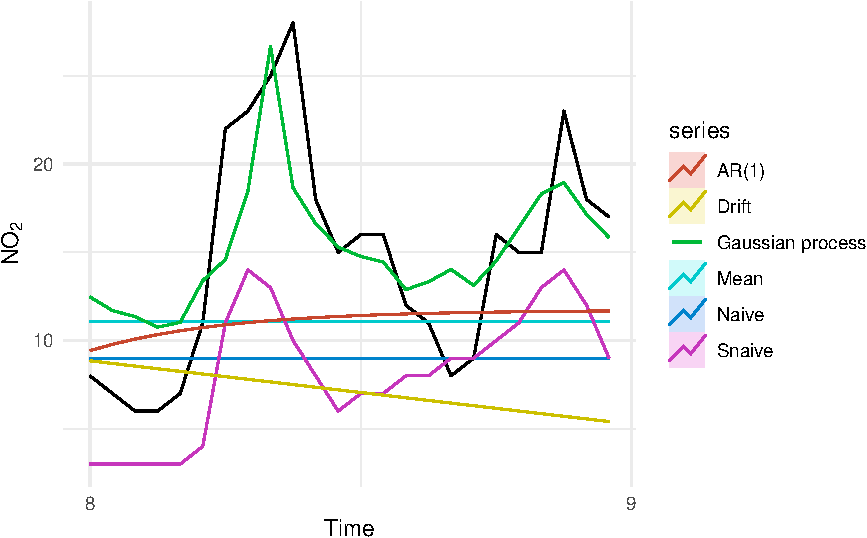
\includegraphics[keepaspectratio]{report_files/figure-latex/Model comparison plots-1.pdf}}
\caption{Time series of the fitted models on the out-of-sample period
06/02/2019 00:00 to 06/02/2019 23:00.}
\end{figure}

\subsection{Cross validation}\label{cross-validation}

Cross-validation was conducted as follows: a period of 7 days from
08/02/2019 at 00:00 to 15/02/2019 at 23:00 was used for the training
set, and one hour on 16/02/2019 at 00:00 was used as a test set. On each
iteration, we increment the training set and shift the test set by one
time point, after which loss functions (MSE, MAE, and MAPE) are
calculated and stored in a matrix. Once all ten iterations are
completed, the error functions are averaged over all iterations.

\begin{figure}
\centering
\pandocbounded{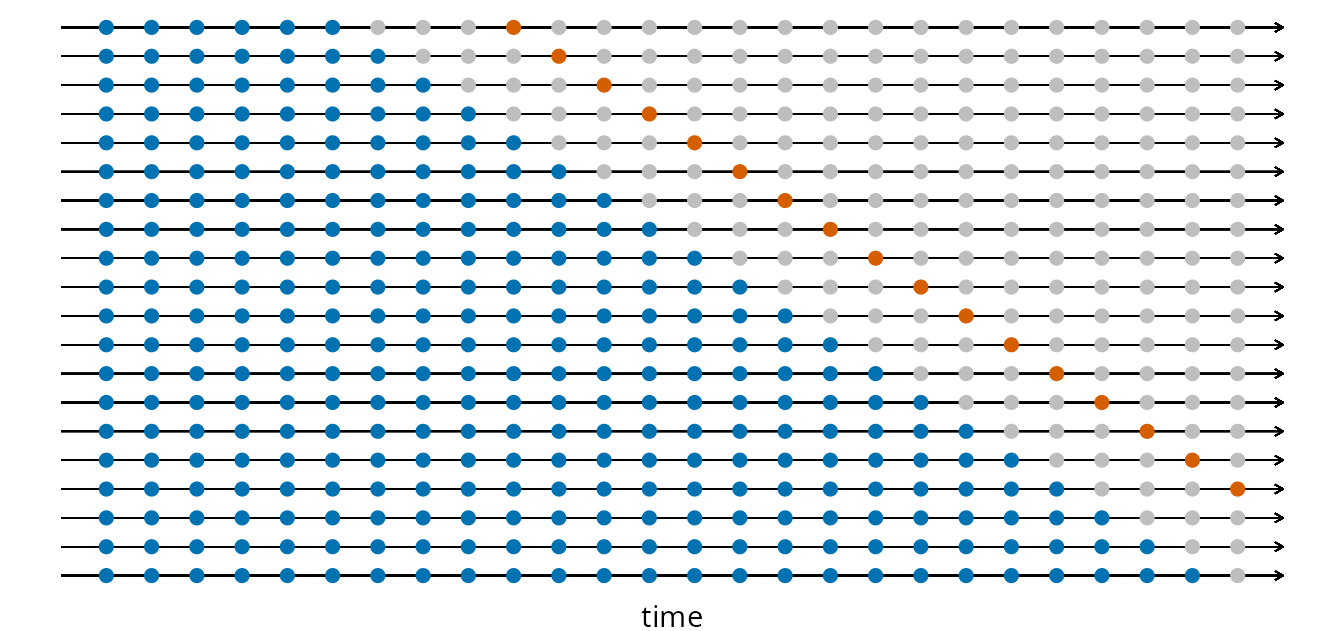
\includegraphics[keepaspectratio]{../images/cross_validation.png}}
\caption{Illustration of the rolling-origin cross-validation scheme,
showing the expanding training set and one-step-ahead test set.}
\end{figure}

\section{Appendix}\label{appendix}

\begin{Shaded}
\begin{Highlighting}[]
\CommentTok{\# Attach the required packages.}
\FunctionTok{require}\NormalTok{(}\AttributeTok{package =} \StringTok{"bayesplot"}\NormalTok{)}
\FunctionTok{require}\NormalTok{(}\AttributeTok{package =} \StringTok{"cmdstanr"}\NormalTok{)}
\FunctionTok{require}\NormalTok{(}\AttributeTok{package =} \StringTok{"corrplot"}\NormalTok{)}
\FunctionTok{require}\NormalTok{(}\AttributeTok{package =} \StringTok{"forecast"}\NormalTok{)}
\FunctionTok{require}\NormalTok{(}\AttributeTok{package =} \StringTok{"ggplot2"}\NormalTok{)}
\FunctionTok{require}\NormalTok{(}\AttributeTok{package =} \StringTok{"kableExtra"}\NormalTok{)}
\FunctionTok{require}\NormalTok{(}\AttributeTok{package =} \StringTok{"knitr"}\NormalTok{)}
\FunctionTok{require}\NormalTok{(}\AttributeTok{package =} \StringTok{"rstan"}\NormalTok{)}
\FunctionTok{require}\NormalTok{(}\AttributeTok{package =} \StringTok{"parallel"}\NormalTok{)}
\FunctionTok{require}\NormalTok{(}\AttributeTok{package =} \StringTok{"posterior"}\NormalTok{)}
\FunctionTok{color\_scheme\_set}\NormalTok{(}\StringTok{"brightblue"}\NormalTok{)}


\CommentTok{\# Load the datasets.}
\FunctionTok{load}\NormalTok{(}\AttributeTok{file =} \StringTok{"../objects/extracted\_data\_storage.RData"}\NormalTok{)}
\FunctionTok{load}\NormalTok{(}\AttributeTok{file =} \StringTok{"../objects/imputed\_data\_storage.RData"}\NormalTok{)}

\CommentTok{\# Extract the datasets.}
\NormalTok{X1 }\OtherTok{\textless{}{-}}\NormalTok{ extracted\_data[[}\DecValTok{1}\NormalTok{]]}
\NormalTok{X2 }\OtherTok{\textless{}{-}}\NormalTok{ imputed\_data[[}\DecValTok{1}\NormalTok{]]}

\CommentTok{\# Declare variable names.}
\NormalTok{var\_name }\OtherTok{\textless{}{-}} \FunctionTok{c}\NormalTok{(}\StringTok{"DateTime"}\NormalTok{, }\StringTok{"NO2"}\NormalTok{, }\StringTok{"PM10"}\NormalTok{, }\StringTok{"SO2"}\NormalTok{, }\StringTok{"Speed"}\NormalTok{)}

\CommentTok{\# Declare variable names in a proper format.}
\NormalTok{x\_name }\OtherTok{\textless{}{-}} \FunctionTok{c}\NormalTok{(}\StringTok{"DateTime"}\NormalTok{, }
            \FunctionTok{expression}\NormalTok{(NO[}\DecValTok{2}\NormalTok{] }\SpecialCharTok{\textasciitilde{}} \StringTok{"("} \SpecialCharTok{*}\NormalTok{ mu }\SpecialCharTok{*} \StringTok{"g/m"}\SpecialCharTok{\^{}}\DecValTok{3} \SpecialCharTok{*} \StringTok{")"}\NormalTok{), }
            \FunctionTok{expression}\NormalTok{(PM[}\DecValTok{10}\NormalTok{] }\SpecialCharTok{\textasciitilde{}} \StringTok{"("} \SpecialCharTok{*}\NormalTok{ mu }\SpecialCharTok{*} \StringTok{"g/m"}\SpecialCharTok{\^{}}\DecValTok{3} \SpecialCharTok{*} \StringTok{")"}\NormalTok{),}
            \FunctionTok{expression}\NormalTok{(SO[}\DecValTok{2}\NormalTok{] }\SpecialCharTok{\textasciitilde{}} \StringTok{"("} \SpecialCharTok{*}\NormalTok{ mu }\SpecialCharTok{*} \StringTok{"g/m"}\SpecialCharTok{\^{}}\DecValTok{3} \SpecialCharTok{*} \StringTok{")"}\NormalTok{), }
            \FunctionTok{expression}\NormalTok{(}\StringTok{"Wind Speed"} \SpecialCharTok{\textasciitilde{}} \StringTok{"(m/s)"}\NormalTok{))}

\CommentTok{\# Calculate summary statistics.}
\NormalTok{summary\_statistics }\OtherTok{\textless{}{-}} \ControlFlowTok{function}\NormalTok{(X)\{}
   \FunctionTok{rbind}\NormalTok{(}\StringTok{"Min."} \OtherTok{=} \FunctionTok{sapply}\NormalTok{(}\AttributeTok{X =}\NormalTok{ X, }\AttributeTok{FUN =}\NormalTok{ min, }\AttributeTok{na.rm =} \ConstantTok{TRUE}\NormalTok{),}
         \StringTok{"1st Qu."} \OtherTok{=} \FunctionTok{sapply}\NormalTok{(}\AttributeTok{X =}\NormalTok{ X, }\AttributeTok{FUN =}\NormalTok{ quantile, }\FloatTok{0.25}\NormalTok{, }\AttributeTok{na.rm =} \ConstantTok{TRUE}\NormalTok{),}
         \StringTok{"Median"} \OtherTok{=} \FunctionTok{sapply}\NormalTok{(}\AttributeTok{X =}\NormalTok{ X, }\AttributeTok{FUN =}\NormalTok{ median, }\AttributeTok{na.rm =} \ConstantTok{TRUE}\NormalTok{),}
         \StringTok{"Mean"} \OtherTok{=} \FunctionTok{sapply}\NormalTok{(}\AttributeTok{X =}\NormalTok{ X, }\AttributeTok{FUN =}\NormalTok{ mean, }\AttributeTok{na.rm =} \ConstantTok{TRUE}\NormalTok{),}
         \StringTok{"SD"} \OtherTok{=} \FunctionTok{sapply}\NormalTok{(}\AttributeTok{X =}\NormalTok{ X, }\AttributeTok{FUN =}\NormalTok{ sd, }\AttributeTok{na.rm =} \ConstantTok{TRUE}\NormalTok{),}
         \StringTok{"3rd Qu."} \OtherTok{=} \FunctionTok{sapply}\NormalTok{(}\AttributeTok{X =}\NormalTok{ X, }\AttributeTok{FUN =}\NormalTok{ quantile, }\FloatTok{0.75}\NormalTok{, }\AttributeTok{na.rm =} \ConstantTok{TRUE}\NormalTok{),}
         \StringTok{"Max."} \OtherTok{=} \FunctionTok{sapply}\NormalTok{(}\AttributeTok{X =}\NormalTok{ X, }\AttributeTok{FUN =}\NormalTok{ max, }\AttributeTok{na.rm =} \ConstantTok{TRUE}\NormalTok{),}
         \StringTok{"NA"} \OtherTok{=} \FunctionTok{sapply}\NormalTok{(}\AttributeTok{X =}\NormalTok{ X, }\AttributeTok{FUN =} \ControlFlowTok{function}\NormalTok{(column) }\FunctionTok{sum}\NormalTok{(}\FunctionTok{is.na}\NormalTok{(column))))}
\NormalTok{\}}
\NormalTok{S\_mat1 }\OtherTok{\textless{}{-}} \FunctionTok{summary\_statistics}\NormalTok{(}\AttributeTok{X =}\NormalTok{ X1)}
\NormalTok{S\_mat2 }\OtherTok{\textless{}{-}} \FunctionTok{summary\_statistics}\NormalTok{(}\AttributeTok{X =}\NormalTok{ X2)}

\CommentTok{\# Display summary statistics.}
\FunctionTok{kable}\NormalTok{(}\AttributeTok{x =} \FunctionTok{round}\NormalTok{(}\AttributeTok{x =} \FunctionTok{t}\NormalTok{(}\AttributeTok{x =}\NormalTok{ S\_mat1[, }\DecValTok{2}\SpecialCharTok{:}\DecValTok{5}\NormalTok{]), }\AttributeTok{digits =} \DecValTok{3}\NormalTok{), }
        \AttributeTok{caption =} \StringTok{"Summary statistics of the air quality dataset from 01/01/2019 to 31/12/2019 measured hourly."}\NormalTok{)}

\FunctionTok{kable}\NormalTok{(}\AttributeTok{x =} \FunctionTok{round}\NormalTok{(}\AttributeTok{x =} \FunctionTok{t}\NormalTok{(}\AttributeTok{x =}\NormalTok{ S\_mat2[, }\DecValTok{2}\SpecialCharTok{:}\DecValTok{5}\NormalTok{]), }\AttributeTok{digits =} \DecValTok{3}\NormalTok{), }
        \AttributeTok{caption =} \StringTok{"Summary statistics of the imputed air quality dataset from 01/01/2019 to 31/12/2019."}\NormalTok{)}

\CommentTok{\# Correlation plot for the original data.}
\FunctionTok{par}\NormalTok{(}\AttributeTok{mfrow =} \FunctionTok{c}\NormalTok{(}\DecValTok{1}\NormalTok{, }\DecValTok{2}\NormalTok{))}
\NormalTok{cor\_mat1 }\OtherTok{\textless{}{-}} \FunctionTok{cor}\NormalTok{(X1[, }\DecValTok{2}\SpecialCharTok{:}\DecValTok{5}\NormalTok{], }\AttributeTok{use =} \StringTok{"na.or.complete"}\NormalTok{, }\AttributeTok{method =} \StringTok{"pearson"}\NormalTok{)}
\FunctionTok{corrplot}\NormalTok{(}\AttributeTok{corr =}\NormalTok{ cor\_mat1, }\AttributeTok{method =} \StringTok{"number"}\NormalTok{, }\AttributeTok{type =} \StringTok{"lower"}\NormalTok{)}

\CommentTok{\# Correlation plot for the imputed data.}
\NormalTok{cor\_mat2 }\OtherTok{\textless{}{-}} \FunctionTok{cor}\NormalTok{(X2[, }\DecValTok{2}\SpecialCharTok{:}\DecValTok{5}\NormalTok{], }\AttributeTok{method =} \StringTok{"pearson"}\NormalTok{)}
\FunctionTok{corrplot}\NormalTok{(}\AttributeTok{corr =}\NormalTok{ cor\_mat2, }\AttributeTok{method =} \StringTok{"number"}\NormalTok{, }\AttributeTok{type =} \StringTok{"lower"}\NormalTok{)}

\CommentTok{\# Function to sketch scatter plots.}
\NormalTok{draw\_plots }\OtherTok{\textless{}{-}} \ControlFlowTok{function}\NormalTok{(X, name)\{}
   \ControlFlowTok{for}\NormalTok{(i }\ControlFlowTok{in} \DecValTok{2}\SpecialCharTok{:}\DecValTok{5}\NormalTok{)\{}
\NormalTok{      filename }\OtherTok{\textless{}{-}} \FunctionTok{paste0}\NormalTok{(}\StringTok{"../images/"}\NormalTok{, name, }\StringTok{"\_"}\NormalTok{, }\FunctionTok{tolower}\NormalTok{(}\AttributeTok{x =}\NormalTok{ var\_name[i]), }\StringTok{".png"}\NormalTok{)}
      \FunctionTok{plot}\NormalTok{(}\AttributeTok{x =}\NormalTok{ X}\SpecialCharTok{$}\NormalTok{DateTime, }\AttributeTok{y =}\NormalTok{ X[[var\_name[i]]], }
           \AttributeTok{main =} \StringTok{""}\NormalTok{, }\AttributeTok{xlab =} \StringTok{"Time"}\NormalTok{, }\AttributeTok{ylab =}\NormalTok{ x\_name[i],}
           \AttributeTok{type =} \StringTok{"l"}\NormalTok{, }\AttributeTok{col =} \StringTok{"steelblue"}\NormalTok{, }\AttributeTok{cex =} \FloatTok{0.5}\NormalTok{)}
\NormalTok{   \}}
\NormalTok{\}}

\CommentTok{\# Scatter plots for the original data.}
\FunctionTok{par}\NormalTok{(}\AttributeTok{mfrow =} \FunctionTok{c}\NormalTok{(}\DecValTok{2}\NormalTok{, }\DecValTok{2}\NormalTok{))}
\FunctionTok{draw\_plots}\NormalTok{(}\AttributeTok{X =}\NormalTok{ X1, }\AttributeTok{name =} \StringTok{"extracted"}\NormalTok{)}

\CommentTok{\# Scatter plots for the imputed data.}
\FunctionTok{par}\NormalTok{(}\AttributeTok{mfrow =} \FunctionTok{c}\NormalTok{(}\DecValTok{2}\NormalTok{, }\DecValTok{2}\NormalTok{))}
\FunctionTok{draw\_plots}\NormalTok{(}\AttributeTok{X =}\NormalTok{ X2, }\AttributeTok{name =} \StringTok{"imputed"}\NormalTok{)}

\CommentTok{\# Load the dataset.}
\FunctionTok{load}\NormalTok{(}\AttributeTok{file =} \StringTok{"../objects/window\_data\_storage.RData"}\NormalTok{)}


\NormalTok{R\_mat }\OtherTok{\textless{}{-}} \FunctionTok{matrix}\NormalTok{(}\AttributeTok{data =} \ConstantTok{NA}\NormalTok{, }\AttributeTok{nrow =} \DecValTok{3}\NormalTok{, }\AttributeTok{ncol =} \DecValTok{6}\NormalTok{, }
                \AttributeTok{dimnames =} \FunctionTok{list}\NormalTok{(}\FunctionTok{c}\NormalTok{(}\StringTok{"RMSE"}\NormalTok{, }\StringTok{"MAE"}\NormalTok{, }\StringTok{"MAPE"}\NormalTok{), }
                                \FunctionTok{c}\NormalTok{(}\StringTok{"Mean"}\NormalTok{, }\StringTok{"Naive"}\NormalTok{, }\StringTok{"Seasonal naive"}\NormalTok{, }\StringTok{"Drift"}\NormalTok{, }\StringTok{"AR(1)"}\NormalTok{, }\StringTok{"Gaussian process"}\NormalTok{)))}

\CommentTok{\# Fit the model(s).}
\NormalTok{mean\_fit }\OtherTok{\textless{}{-}} \FunctionTok{meanf}\NormalTok{(}\AttributeTok{y =}\NormalTok{ y1, }\AttributeTok{h =}\NormalTok{ h)}
\NormalTok{naive\_fit }\OtherTok{\textless{}{-}} \FunctionTok{naive}\NormalTok{(}\AttributeTok{y =}\NormalTok{ y1, }\AttributeTok{h =}\NormalTok{ h)}
\NormalTok{snaive\_fit }\OtherTok{\textless{}{-}} \FunctionTok{snaive}\NormalTok{(}\AttributeTok{y =}\NormalTok{ y1, }\AttributeTok{h =}\NormalTok{ h)}
\NormalTok{drift\_fit }\OtherTok{\textless{}{-}} \FunctionTok{rwf}\NormalTok{(}\AttributeTok{y =}\NormalTok{ y1, }\AttributeTok{h =}\NormalTok{ h, }\AttributeTok{drift =} \ConstantTok{TRUE}\NormalTok{)}
\NormalTok{arima\_obj }\OtherTok{\textless{}{-}} \FunctionTok{arima}\NormalTok{(}\AttributeTok{x =}\NormalTok{ y1, }\AttributeTok{order =} \FunctionTok{c}\NormalTok{(}\DecValTok{1}\NormalTok{, }\DecValTok{0}\NormalTok{, }\DecValTok{0}\NormalTok{))}
\NormalTok{arima\_fit }\OtherTok{\textless{}{-}} \FunctionTok{forecast}\NormalTok{(}\AttributeTok{object =}\NormalTok{ arima\_obj, }\AttributeTok{h =}\NormalTok{ h)}

\CommentTok{\# Calculate the mean square error.}
\NormalTok{R\_mat[}\DecValTok{1}\NormalTok{, }\DecValTok{1}\NormalTok{] }\OtherTok{\textless{}{-}} \FunctionTok{sqrt}\NormalTok{(}\FunctionTok{mean}\NormalTok{((mean\_fit}\SpecialCharTok{$}\NormalTok{mean }\SpecialCharTok{{-}}\NormalTok{ y2)}\SpecialCharTok{\^{}}\DecValTok{2}\NormalTok{))}
\NormalTok{R\_mat[}\DecValTok{1}\NormalTok{, }\DecValTok{2}\NormalTok{] }\OtherTok{\textless{}{-}} \FunctionTok{sqrt}\NormalTok{(}\FunctionTok{mean}\NormalTok{((naive\_fit}\SpecialCharTok{$}\NormalTok{mean }\SpecialCharTok{{-}}\NormalTok{ y2)}\SpecialCharTok{\^{}}\DecValTok{2}\NormalTok{))}
\NormalTok{R\_mat[}\DecValTok{1}\NormalTok{, }\DecValTok{3}\NormalTok{] }\OtherTok{\textless{}{-}} \FunctionTok{sqrt}\NormalTok{(}\FunctionTok{mean}\NormalTok{((snaive\_fit}\SpecialCharTok{$}\NormalTok{mean }\SpecialCharTok{{-}}\NormalTok{ y2)}\SpecialCharTok{\^{}}\DecValTok{2}\NormalTok{))}
\NormalTok{R\_mat[}\DecValTok{1}\NormalTok{, }\DecValTok{4}\NormalTok{] }\OtherTok{\textless{}{-}} \FunctionTok{sqrt}\NormalTok{(}\FunctionTok{mean}\NormalTok{((drift\_fit}\SpecialCharTok{$}\NormalTok{mean }\SpecialCharTok{{-}}\NormalTok{ y2)}\SpecialCharTok{\^{}}\DecValTok{2}\NormalTok{))}
\NormalTok{R\_mat[}\DecValTok{1}\NormalTok{, }\DecValTok{5}\NormalTok{] }\OtherTok{\textless{}{-}} \FunctionTok{sqrt}\NormalTok{(}\FunctionTok{mean}\NormalTok{((arima\_fit}\SpecialCharTok{$}\NormalTok{mean }\SpecialCharTok{{-}}\NormalTok{ y2)}\SpecialCharTok{\^{}}\DecValTok{2}\NormalTok{))}

\CommentTok{\# Calculate the mean absolute error.}
\NormalTok{R\_mat[}\DecValTok{2}\NormalTok{, }\DecValTok{1}\NormalTok{] }\OtherTok{\textless{}{-}} \FunctionTok{mean}\NormalTok{(}\FunctionTok{abs}\NormalTok{(mean\_fit}\SpecialCharTok{$}\NormalTok{mean }\SpecialCharTok{{-}}\NormalTok{ y2))}
\NormalTok{R\_mat[}\DecValTok{2}\NormalTok{, }\DecValTok{2}\NormalTok{] }\OtherTok{\textless{}{-}} \FunctionTok{mean}\NormalTok{(}\FunctionTok{abs}\NormalTok{(naive\_fit}\SpecialCharTok{$}\NormalTok{mean }\SpecialCharTok{{-}}\NormalTok{ y2))}
\NormalTok{R\_mat[}\DecValTok{2}\NormalTok{, }\DecValTok{3}\NormalTok{] }\OtherTok{\textless{}{-}} \FunctionTok{mean}\NormalTok{(}\FunctionTok{abs}\NormalTok{(snaive\_fit}\SpecialCharTok{$}\NormalTok{mean }\SpecialCharTok{{-}}\NormalTok{ y2))}
\NormalTok{R\_mat[}\DecValTok{2}\NormalTok{, }\DecValTok{4}\NormalTok{] }\OtherTok{\textless{}{-}} \FunctionTok{mean}\NormalTok{(}\FunctionTok{abs}\NormalTok{(drift\_fit}\SpecialCharTok{$}\NormalTok{mean }\SpecialCharTok{{-}}\NormalTok{ y2))}
\NormalTok{R\_mat[}\DecValTok{2}\NormalTok{, }\DecValTok{5}\NormalTok{] }\OtherTok{\textless{}{-}} \FunctionTok{mean}\NormalTok{(}\FunctionTok{abs}\NormalTok{(arima\_fit}\SpecialCharTok{$}\NormalTok{mean }\SpecialCharTok{{-}}\NormalTok{ y2))}

\CommentTok{\# Calculate the mean absolute percentage error.}
\NormalTok{R\_mat[}\DecValTok{3}\NormalTok{, }\DecValTok{1}\NormalTok{] }\OtherTok{\textless{}{-}} \FunctionTok{mean}\NormalTok{((}\FunctionTok{abs}\NormalTok{(mean\_fit}\SpecialCharTok{$}\NormalTok{mean }\SpecialCharTok{{-}}\NormalTok{ y2) }\SpecialCharTok{/} \FunctionTok{abs}\NormalTok{(y2)) }\SpecialCharTok{*} \DecValTok{100}\NormalTok{)}
\NormalTok{R\_mat[}\DecValTok{3}\NormalTok{, }\DecValTok{2}\NormalTok{] }\OtherTok{\textless{}{-}} \FunctionTok{mean}\NormalTok{((}\FunctionTok{abs}\NormalTok{(naive\_fit}\SpecialCharTok{$}\NormalTok{mean }\SpecialCharTok{{-}}\NormalTok{ y2) }\SpecialCharTok{/} \FunctionTok{abs}\NormalTok{(y2)) }\SpecialCharTok{*} \DecValTok{100}\NormalTok{)}
\NormalTok{R\_mat[}\DecValTok{3}\NormalTok{, }\DecValTok{3}\NormalTok{] }\OtherTok{\textless{}{-}} \FunctionTok{mean}\NormalTok{((}\FunctionTok{abs}\NormalTok{(snaive\_fit}\SpecialCharTok{$}\NormalTok{mean }\SpecialCharTok{{-}}\NormalTok{ y2) }\SpecialCharTok{/} \FunctionTok{abs}\NormalTok{(y2)) }\SpecialCharTok{*} \DecValTok{100}\NormalTok{)}
\NormalTok{R\_mat[}\DecValTok{3}\NormalTok{, }\DecValTok{4}\NormalTok{] }\OtherTok{\textless{}{-}} \FunctionTok{mean}\NormalTok{((}\FunctionTok{abs}\NormalTok{(drift\_fit}\SpecialCharTok{$}\NormalTok{mean }\SpecialCharTok{{-}}\NormalTok{ y2) }\SpecialCharTok{/} \FunctionTok{abs}\NormalTok{(y2)) }\SpecialCharTok{*} \DecValTok{100}\NormalTok{)}
\NormalTok{R\_mat[}\DecValTok{3}\NormalTok{, }\DecValTok{5}\NormalTok{] }\OtherTok{\textless{}{-}} \FunctionTok{mean}\NormalTok{((}\FunctionTok{abs}\NormalTok{(arima\_fit}\SpecialCharTok{$}\NormalTok{mean }\SpecialCharTok{{-}}\NormalTok{ y2) }\SpecialCharTok{/} \FunctionTok{abs}\NormalTok{(y2)) }\SpecialCharTok{*} \DecValTok{100}\NormalTok{)}

\CommentTok{\# Plot the forecasts.}
\NormalTok{p2 }\OtherTok{\textless{}{-}}\NormalTok{ p2 }\SpecialCharTok{+} \FunctionTok{autolayer}\NormalTok{(}\AttributeTok{object =}\NormalTok{ mean\_fit, }\AttributeTok{series =} \StringTok{"Mean"}\NormalTok{, }\AttributeTok{PI =} \ConstantTok{FALSE}\NormalTok{)}
\NormalTok{p2 }\OtherTok{\textless{}{-}}\NormalTok{ p2 }\SpecialCharTok{+} \FunctionTok{autolayer}\NormalTok{(}\AttributeTok{object =}\NormalTok{ naive\_fit, }\AttributeTok{series =} \StringTok{"Naive"}\NormalTok{, }\AttributeTok{PI =} \ConstantTok{FALSE}\NormalTok{)}
\NormalTok{p2 }\OtherTok{\textless{}{-}}\NormalTok{ p2 }\SpecialCharTok{+} \FunctionTok{autolayer}\NormalTok{(}\AttributeTok{object =}\NormalTok{ snaive\_fit, }\AttributeTok{series =} \StringTok{"Snaive"}\NormalTok{, }\AttributeTok{PI =} \ConstantTok{FALSE}\NormalTok{)}
\NormalTok{p2 }\OtherTok{\textless{}{-}}\NormalTok{ p2 }\SpecialCharTok{+} \FunctionTok{autolayer}\NormalTok{(}\AttributeTok{object =}\NormalTok{ drift\_fit, }\AttributeTok{series =} \StringTok{"Drift"}\NormalTok{, }\AttributeTok{PI =} \ConstantTok{FALSE}\NormalTok{)}
\NormalTok{p2 }\OtherTok{\textless{}{-}}\NormalTok{ p2 }\SpecialCharTok{+} \FunctionTok{autolayer}\NormalTok{(}\AttributeTok{object =}\NormalTok{ arima\_fit, }\AttributeTok{series =} \StringTok{"AR(1)"}\NormalTok{, }\AttributeTok{PI =} \ConstantTok{FALSE}\NormalTok{)}

\NormalTok{cores\_number }\OtherTok{\textless{}{-}} \FunctionTok{detectCores}\NormalTok{() }\SpecialCharTok{{-}} \DecValTok{2}
\NormalTok{stan\_data }\OtherTok{\textless{}{-}} \FunctionTok{list}\NormalTok{(}\AttributeTok{X1 =}\NormalTok{ X1, }\AttributeTok{y1 =}\NormalTok{ y1, }\AttributeTok{n1 =}\NormalTok{ n1, }\AttributeTok{p =}\NormalTok{ p, }\AttributeTok{X2 =}\NormalTok{ X2, }\AttributeTok{n2 =}\NormalTok{ n2)}

\CommentTok{\# Compile Stan model once.}
\NormalTok{mod }\OtherTok{\textless{}{-}} \FunctionTok{cmdstan\_model}\NormalTok{(}\AttributeTok{stan\_file =} \StringTok{"squared\_exponential.stan"}\NormalTok{)}

\CommentTok{\# Sample from a Gaussian process.}
\NormalTok{fit }\OtherTok{\textless{}{-}}\NormalTok{ mod}\SpecialCharTok{$}\FunctionTok{sample}\NormalTok{(}
    \AttributeTok{data =}\NormalTok{ stan\_data,}
   \AttributeTok{chains =} \DecValTok{4}\NormalTok{,}
   \AttributeTok{parallel\_chains =}\NormalTok{ cores\_number,}
   \AttributeTok{seed =} \DecValTok{2025}\NormalTok{,}
   \AttributeTok{refresh =} \DecValTok{0}\NormalTok{,}
   \AttributeTok{show\_messages =} \ConstantTok{FALSE}\NormalTok{,}
    \AttributeTok{show\_exceptions =} \ConstantTok{FALSE}\NormalTok{)}

\CommentTok{\# fit is a CmdStanMCMC object.}
\NormalTok{y2\_draws }\OtherTok{\textless{}{-}}\NormalTok{ fit}\SpecialCharTok{$}\FunctionTok{draws}\NormalTok{(}\StringTok{"y2"}\NormalTok{, }\AttributeTok{format =} \StringTok{"matrix"}\NormalTok{)}
\NormalTok{y2\_mean  }\OtherTok{\textless{}{-}} \FunctionTok{colMeans}\NormalTok{(y2\_draws)}

\NormalTok{y2\_hat }\OtherTok{\textless{}{-}} \FunctionTok{ts}\NormalTok{(y2\_mean, }\AttributeTok{start =} \FunctionTok{start}\NormalTok{(y2), }\AttributeTok{frequency =} \FunctionTok{frequency}\NormalTok{(y2))}

\CommentTok{\# Calculate the error.}
\NormalTok{R\_mat[}\DecValTok{1}\NormalTok{, }\DecValTok{6}\NormalTok{] }\OtherTok{\textless{}{-}} \FunctionTok{sqrt}\NormalTok{(}\FunctionTok{mean}\NormalTok{((y2\_hat }\SpecialCharTok{{-}}\NormalTok{ y2)}\SpecialCharTok{\^{}}\DecValTok{2}\NormalTok{))}
\NormalTok{R\_mat[}\DecValTok{2}\NormalTok{, }\DecValTok{6}\NormalTok{] }\OtherTok{\textless{}{-}} \FunctionTok{mean}\NormalTok{(}\FunctionTok{abs}\NormalTok{(y2\_hat }\SpecialCharTok{{-}}\NormalTok{ y2))}
\NormalTok{R\_mat[}\DecValTok{3}\NormalTok{, }\DecValTok{6}\NormalTok{] }\OtherTok{\textless{}{-}} \FunctionTok{mean}\NormalTok{((}\FunctionTok{abs}\NormalTok{(y2\_hat }\SpecialCharTok{{-}}\NormalTok{ y2) }\SpecialCharTok{/} \FunctionTok{abs}\NormalTok{(y2)) }\SpecialCharTok{*} \DecValTok{100}\NormalTok{)}
\FunctionTok{kable}\NormalTok{(}\AttributeTok{x =} \FunctionTok{t}\NormalTok{(}\FunctionTok{round}\NormalTok{(}\AttributeTok{x =}\NormalTok{ R\_mat, }\AttributeTok{digits =} \DecValTok{3}\NormalTok{)), }
        \AttributeTok{caption =} \StringTok{"Average performance of the fitted models on the out{-}of{-}sample period 16/02/2019 00:00 to 16/02/2019 23:00."}\NormalTok{)}

\CommentTok{\# Plot the forecasts.}
\NormalTok{p2 }\OtherTok{\textless{}{-}}\NormalTok{ p2 }\SpecialCharTok{+} \FunctionTok{autolayer}\NormalTok{(}\AttributeTok{object =}\NormalTok{ y2\_hat, }\AttributeTok{series =} \StringTok{"Gaussian process"}\NormalTok{)}
\NormalTok{p2}
\end{Highlighting}
\end{Shaded}

\begin{Shaded}
\begin{Highlighting}[]
\KeywordTok{functions}\NormalTok{ \{}
  \DataTypeTok{matrix}\NormalTok{ se\_kernel(}\DataTypeTok{matrix}\NormalTok{ X1, }\DataTypeTok{matrix}\NormalTok{ X2, }\DataTypeTok{real}\NormalTok{ alpha, }\DataTypeTok{real}\NormalTok{ rho) \{}
    \DataTypeTok{int}\NormalTok{ n1 = rows(X1);}
    \DataTypeTok{int}\NormalTok{ n2 = rows(X2);}
    \DataTypeTok{matrix}\NormalTok{[n1, n2] K;}

    \ControlFlowTok{for}\NormalTok{ (i }\ControlFlowTok{in} \DecValTok{1}\NormalTok{:n1) \{}
      \ControlFlowTok{for}\NormalTok{ (j }\ControlFlowTok{in} \DecValTok{1}\NormalTok{:n2) \{}
        \CommentTok{// squared Euclidean distance between rows i and j}
        \DataTypeTok{real}\NormalTok{ sqdist = dot\_self(X1[i] {-} X2[j]);}
\NormalTok{        K[i, j] = square(alpha) * exp({-}}\FloatTok{0.5}\NormalTok{ * sqdist / square(rho));}
\NormalTok{      \}}
\NormalTok{    \}}
    \ControlFlowTok{return}\NormalTok{ K;}
\NormalTok{  \}}
\NormalTok{\}}

\KeywordTok{data}\NormalTok{ \{}
  \DataTypeTok{int}\NormalTok{\textless{}}\KeywordTok{lower}\NormalTok{=}\DecValTok{1}\NormalTok{\textgreater{} n1;}
  \DataTypeTok{int}\NormalTok{\textless{}}\KeywordTok{lower}\NormalTok{=}\DecValTok{1}\NormalTok{\textgreater{} p;}
  \DataTypeTok{matrix}\NormalTok{[n1, p] X1;}
  \DataTypeTok{vector}\NormalTok{[n1] y1;}

  \DataTypeTok{int}\NormalTok{\textless{}}\KeywordTok{lower}\NormalTok{=}\DecValTok{1}\NormalTok{\textgreater{} n2;}
  \DataTypeTok{matrix}\NormalTok{[n2, p] X2;}
\NormalTok{\}}

\KeywordTok{transformed data}\NormalTok{ \{}
  \DataTypeTok{real}\NormalTok{ delta = }\FloatTok{1e{-}9}\NormalTok{;}
\NormalTok{\}}

\KeywordTok{parameters}\NormalTok{ \{}
  \DataTypeTok{real}\NormalTok{\textless{}}\KeywordTok{lower}\NormalTok{=}\DecValTok{0}\NormalTok{\textgreater{} alpha;}
  \DataTypeTok{real}\NormalTok{\textless{}}\KeywordTok{lower}\NormalTok{=}\DecValTok{0}\NormalTok{\textgreater{} rho;}
  \DataTypeTok{vector}\NormalTok{[p] beta;}
\NormalTok{\}}

\KeywordTok{model}\NormalTok{ \{}
  \CommentTok{// Priors}
\NormalTok{  alpha \textasciitilde{} normal(}\DecValTok{0}\NormalTok{, }\DecValTok{1}\NormalTok{);}
\NormalTok{  rho \textasciitilde{} normal(}\DecValTok{24}\NormalTok{, }\DecValTok{12}\NormalTok{); }\CommentTok{// half{-}normal since \textless{}lower=0\textgreater{}}
\NormalTok{  beta \textasciitilde{} normal(}\DecValTok{0}\NormalTok{, }\DecValTok{1}\NormalTok{);}

  \CommentTok{// Build covariance for training}
  \DataTypeTok{matrix}\NormalTok{[n1, n1] K11 = se\_kernel(X1, X1, alpha, rho)}
\NormalTok{                       + diag\_matrix(rep\_vector(delta, n1));}
  \DataTypeTok{vector}\NormalTok{[n1] mu1 = X1 * beta;}

  \CommentTok{// Likelihood}
\NormalTok{  y1 \textasciitilde{} multi\_normal(mu1, K11);}
\NormalTok{\}}

\KeywordTok{generated quantities}\NormalTok{ \{}
  \DataTypeTok{vector}\NormalTok{[n2] y2;}

  \CommentTok{// Covariance blocks}
  \DataTypeTok{matrix}\NormalTok{[n1, n1] K11 = se\_kernel(X1, X1, alpha, rho)}
\NormalTok{                       + diag\_matrix(rep\_vector(delta, n1));}
  \DataTypeTok{matrix}\NormalTok{[n1, n2] K12 = se\_kernel(X1, X2, alpha, rho);}
  \DataTypeTok{matrix}\NormalTok{[n2, n2] K22 = se\_kernel(X2, X2, alpha, rho)}
\NormalTok{                       + diag\_matrix(rep\_vector(delta, n2));}

  \CommentTok{// Means}
  \DataTypeTok{vector}\NormalTok{[n1] mu1 = X1 * beta;}
  \DataTypeTok{vector}\NormalTok{[n2] mu2 = X2 * beta;}

  \CommentTok{// Cholesky factor of K11}
  \DataTypeTok{matrix}\NormalTok{[n1, n1] L = cholesky\_decompose(K11);}

  \CommentTok{// Predictive mean}
  \DataTypeTok{vector}\NormalTok{[n1] y1\_centered = y1 {-} mu1;}
  \DataTypeTok{vector}\NormalTok{[n1] v = mdivide\_left\_tri\_low(L, y1\_centered);}
  \DataTypeTok{vector}\NormalTok{[n1] w = mdivide\_right\_tri\_low(v\textquotesingle{}, L)\textquotesingle{};}
  \DataTypeTok{vector}\NormalTok{[n2] pred\_mean = mu2 + K12\textquotesingle{} * w;}

  \CommentTok{// Predictive covariance}
  \DataTypeTok{matrix}\NormalTok{[n1, n2] A = mdivide\_left\_tri\_low(L, K12);}
  \DataTypeTok{matrix}\NormalTok{[n2, n2] pred\_cov = K22 {-} A\textquotesingle{} * A;}

  \CommentTok{// Draw sample}
\NormalTok{  y2 = multi\_normal\_rng(pred\_mean, pred\_cov);}
\NormalTok{\}}
\end{Highlighting}
\end{Shaded}

\section*{References}\label{references}
\addcontentsline{toc}{section}{References}

\phantomsection\label{refs}
\begin{CSLReferences}{1}{0}
\bibitem[\citeproctext]{ref-CityofCapeTown2015}
Cape Town, City of. 2015. {``Open Data Portal.''}
\url{https://odp-cctegis.opendata.arcgis.com/}.

\bibitem[\citeproctext]{ref-CityofCapeTown2024}
---------. 2024. {``Air Quality Management Plan.''}
\url{https://resource.capetown.gov.za/documentcentre/Documents/City\%20strategies,\%20plans\%20and\%20frameworks/Air_Quality_Management_Plan_2024.pdf}.

\end{CSLReferences}

\end{document}
